\documentclass{article}


\usepackage{graphicx}  %  allow import images
\usepackage{float}         %  allows controlling float position
\usepackage{subfig}



\begin{document}
	
%	Here comes the text
%	\begin{figure}[H]
%	\centering
%	\includegraphics[height=3in]{/Users/asamad/Desktop/latex/article/fig/saf_2.jpg}
%	\caption[Optional Caption1]{Real, Local Caption}
%	\label{fig:Safaa,The Lion}
%\end{figure}

mages is starting somehwere below....
\begin{figure}[H]
	\centering
	\includegraphics[height=3in, angle=-30]{/Users/asamad/Documents/programming_Coding/latex/1_first_course/myimages/saf.png}
	\caption{Safaa The Lion}
	
\end{figure}

After this figure, I'm going to insert another figure:

\begin{figure}[b]
	\centering
	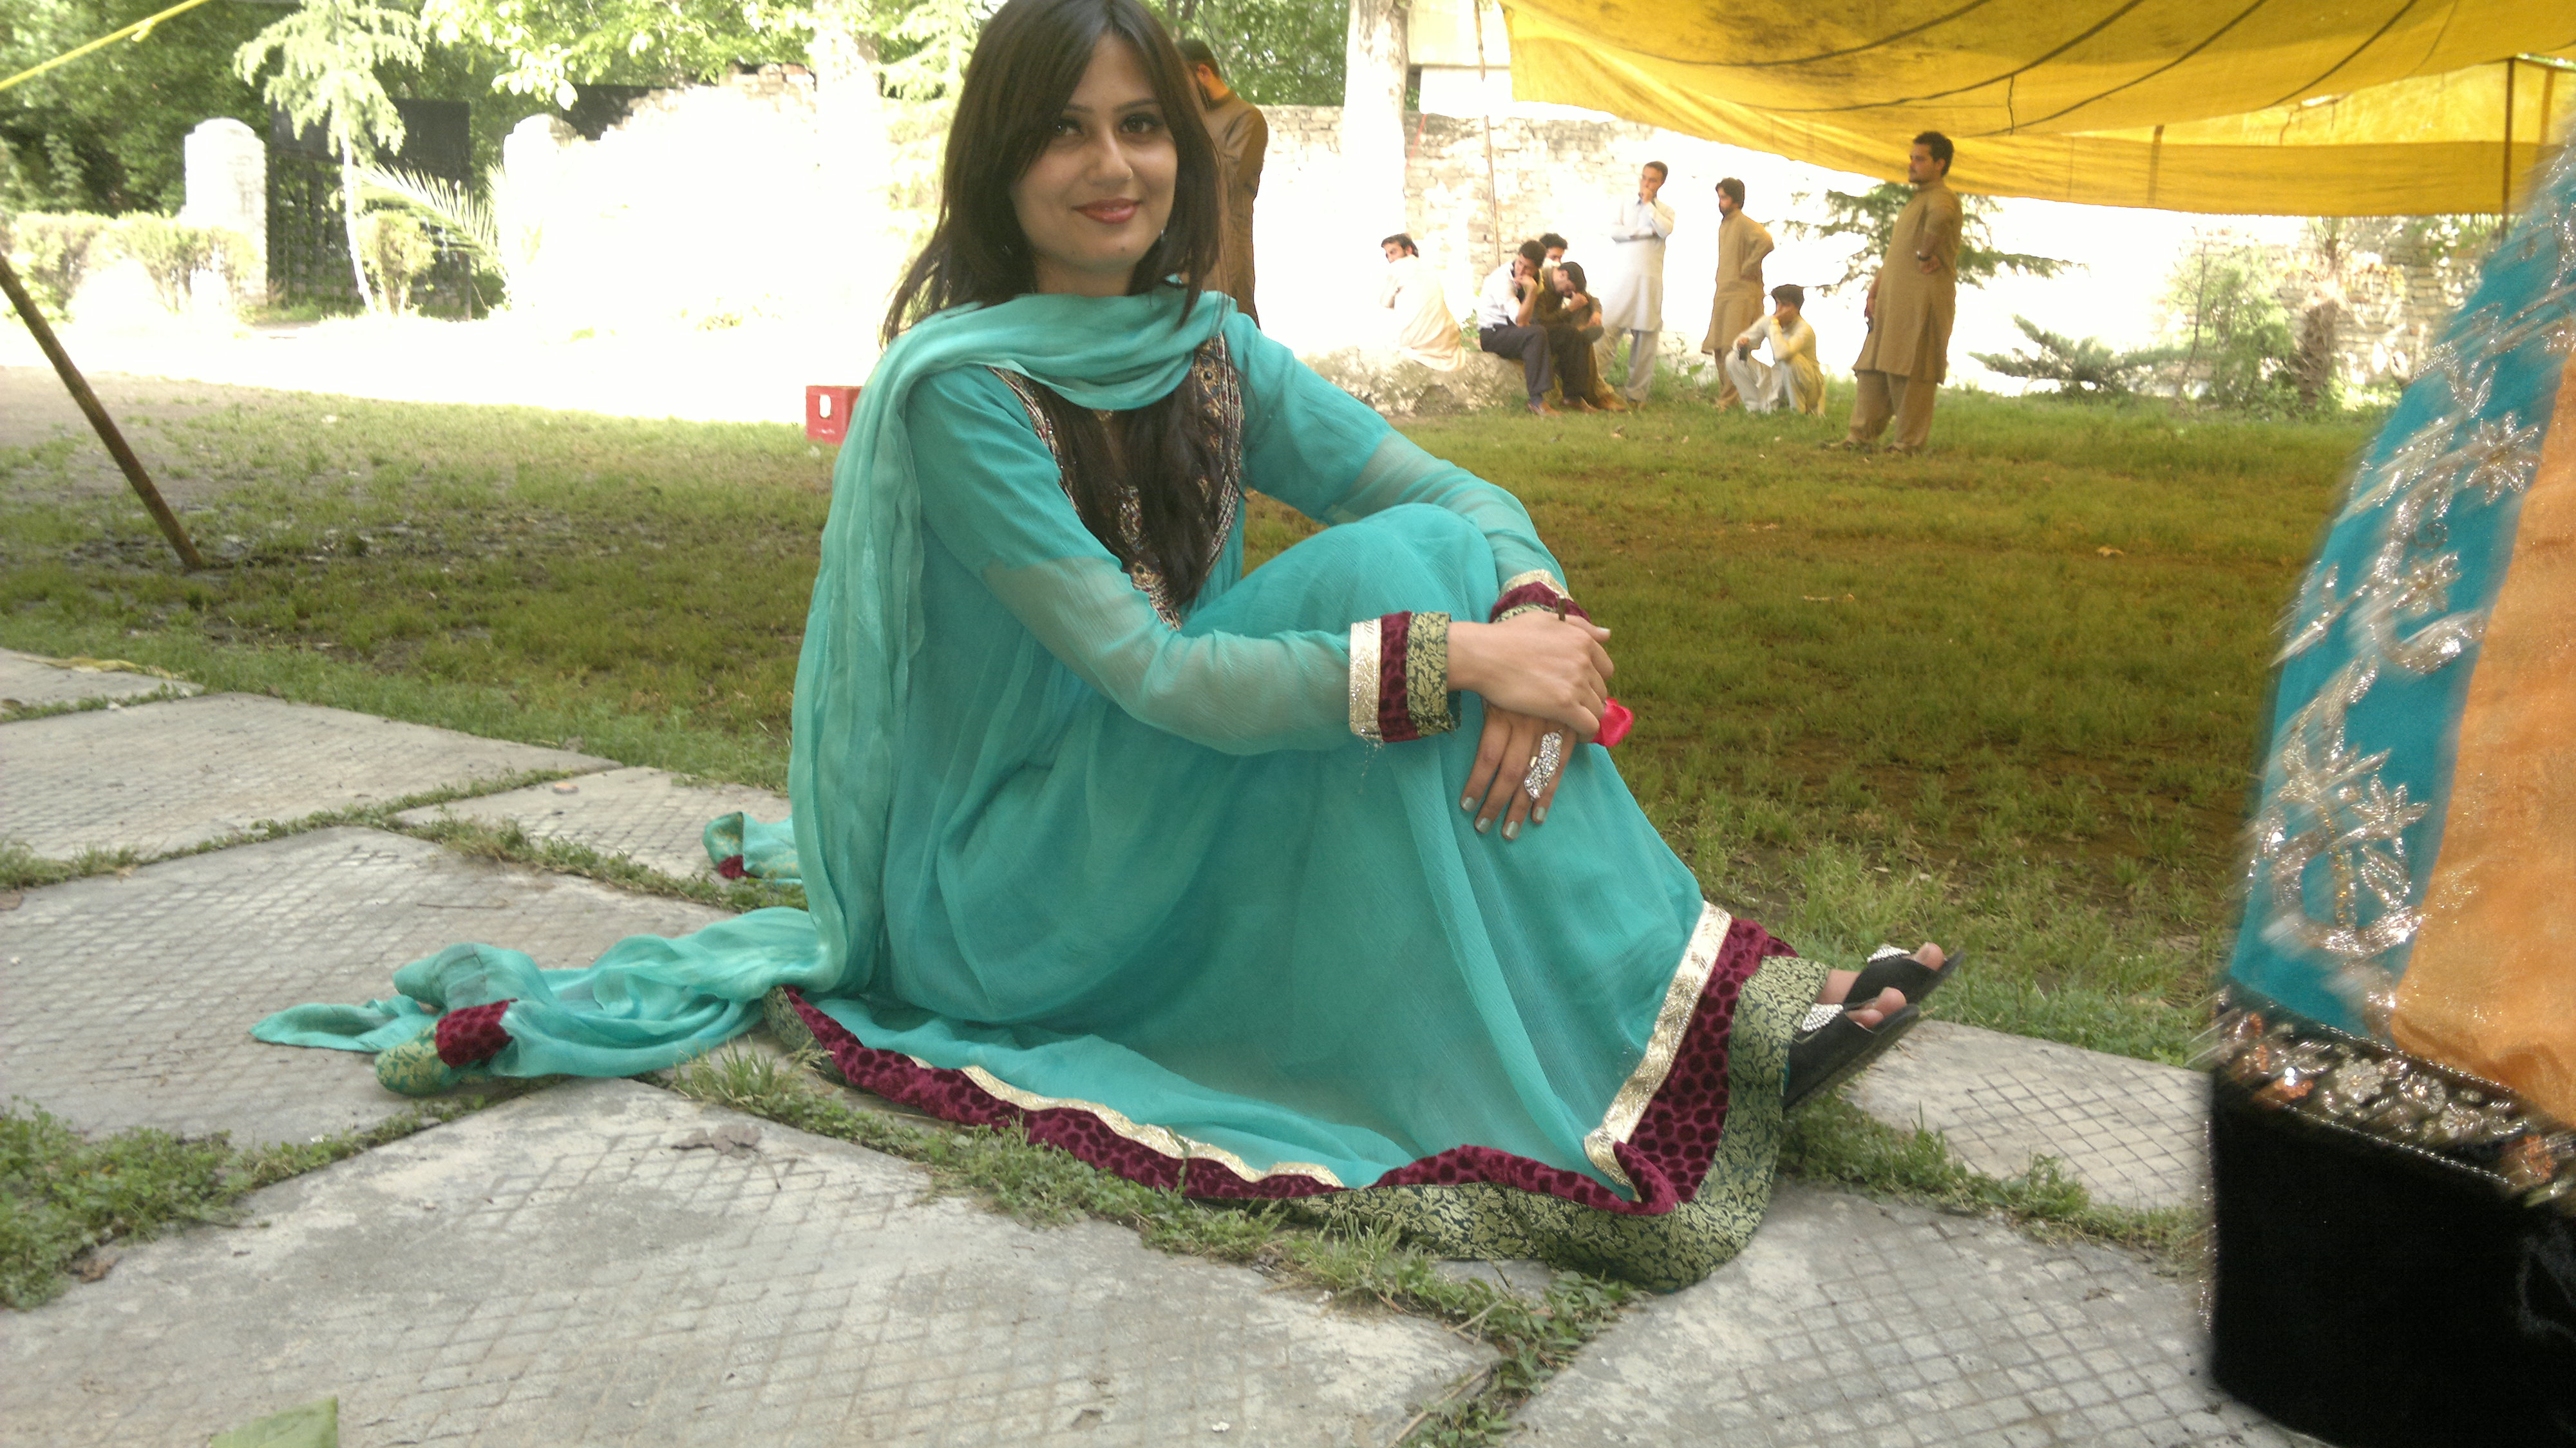
\includegraphics[height=4in]{/Users/asamad/Documents/programming_Coding/latex/1_first_course/myimages/zz3z.jpg}
	\caption{A scan image}
\end{figure}


\begin{figure}[b]
	\centering
	\subfloat{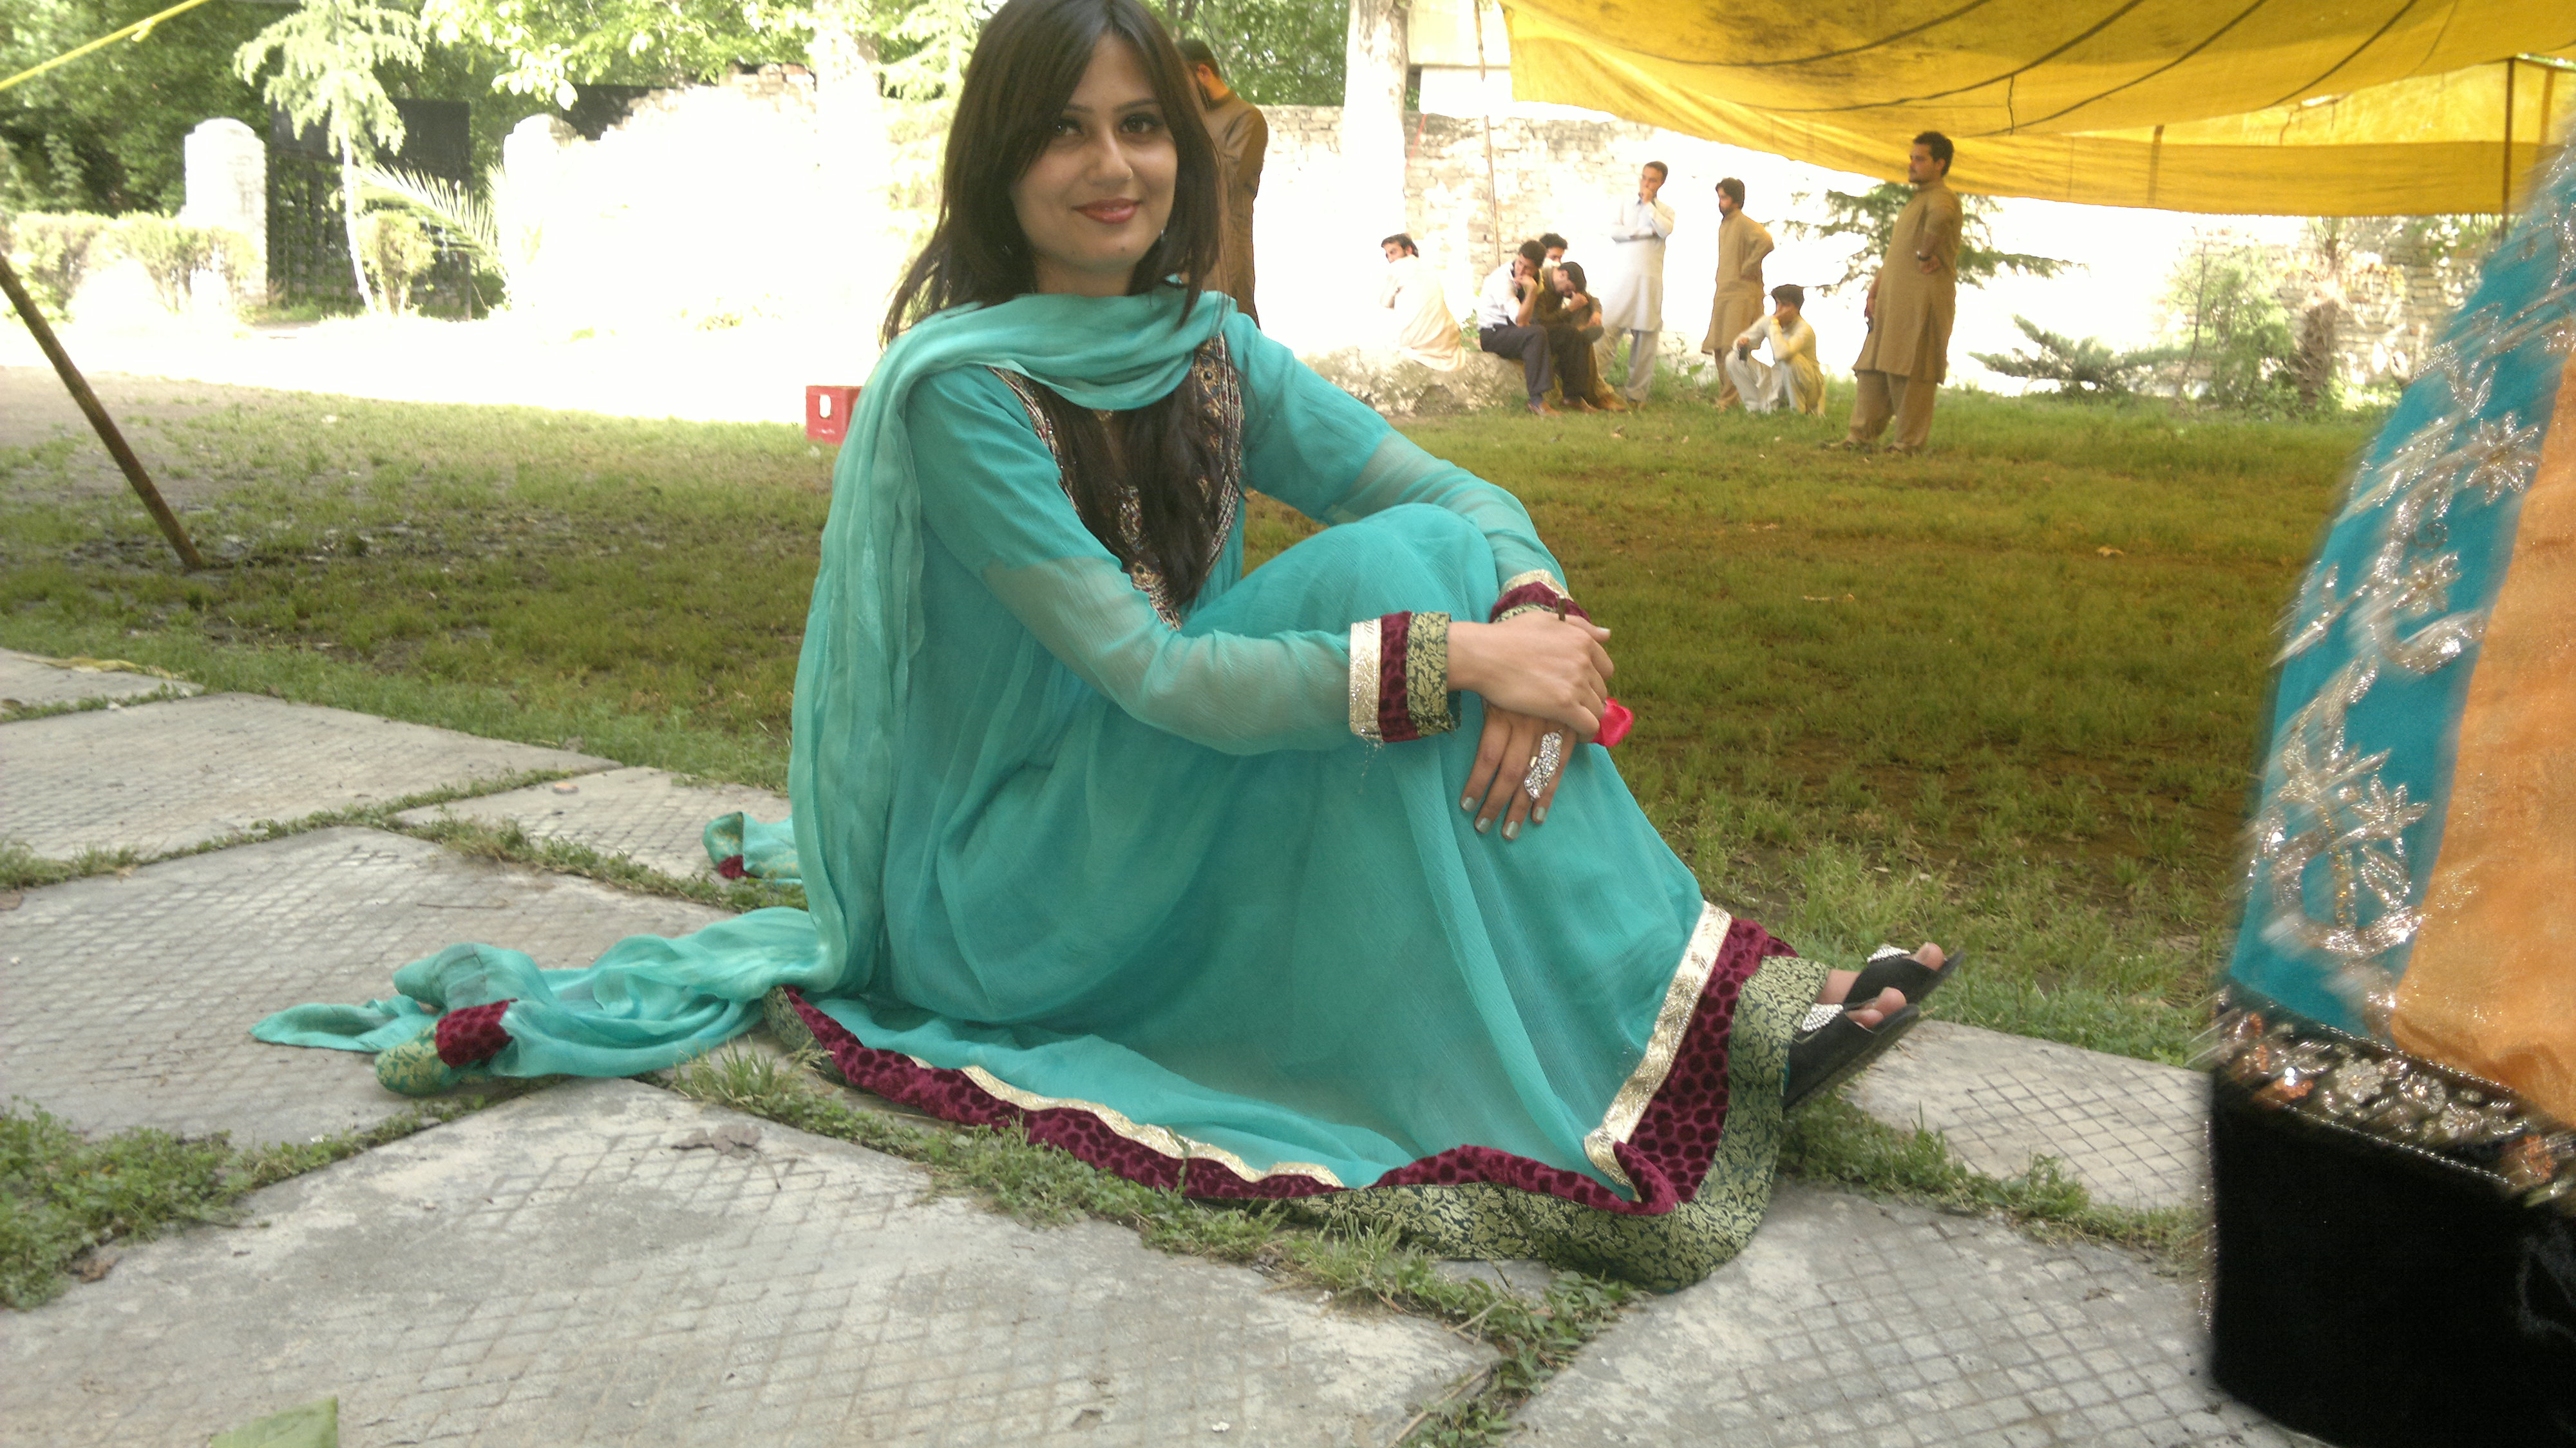
\includegraphics[width=0.5\textwidth]{/Users/asamad/Documents/programming_Coding/latex/1_first_course/myimages/zz3z.jpg}}
	\subfloat{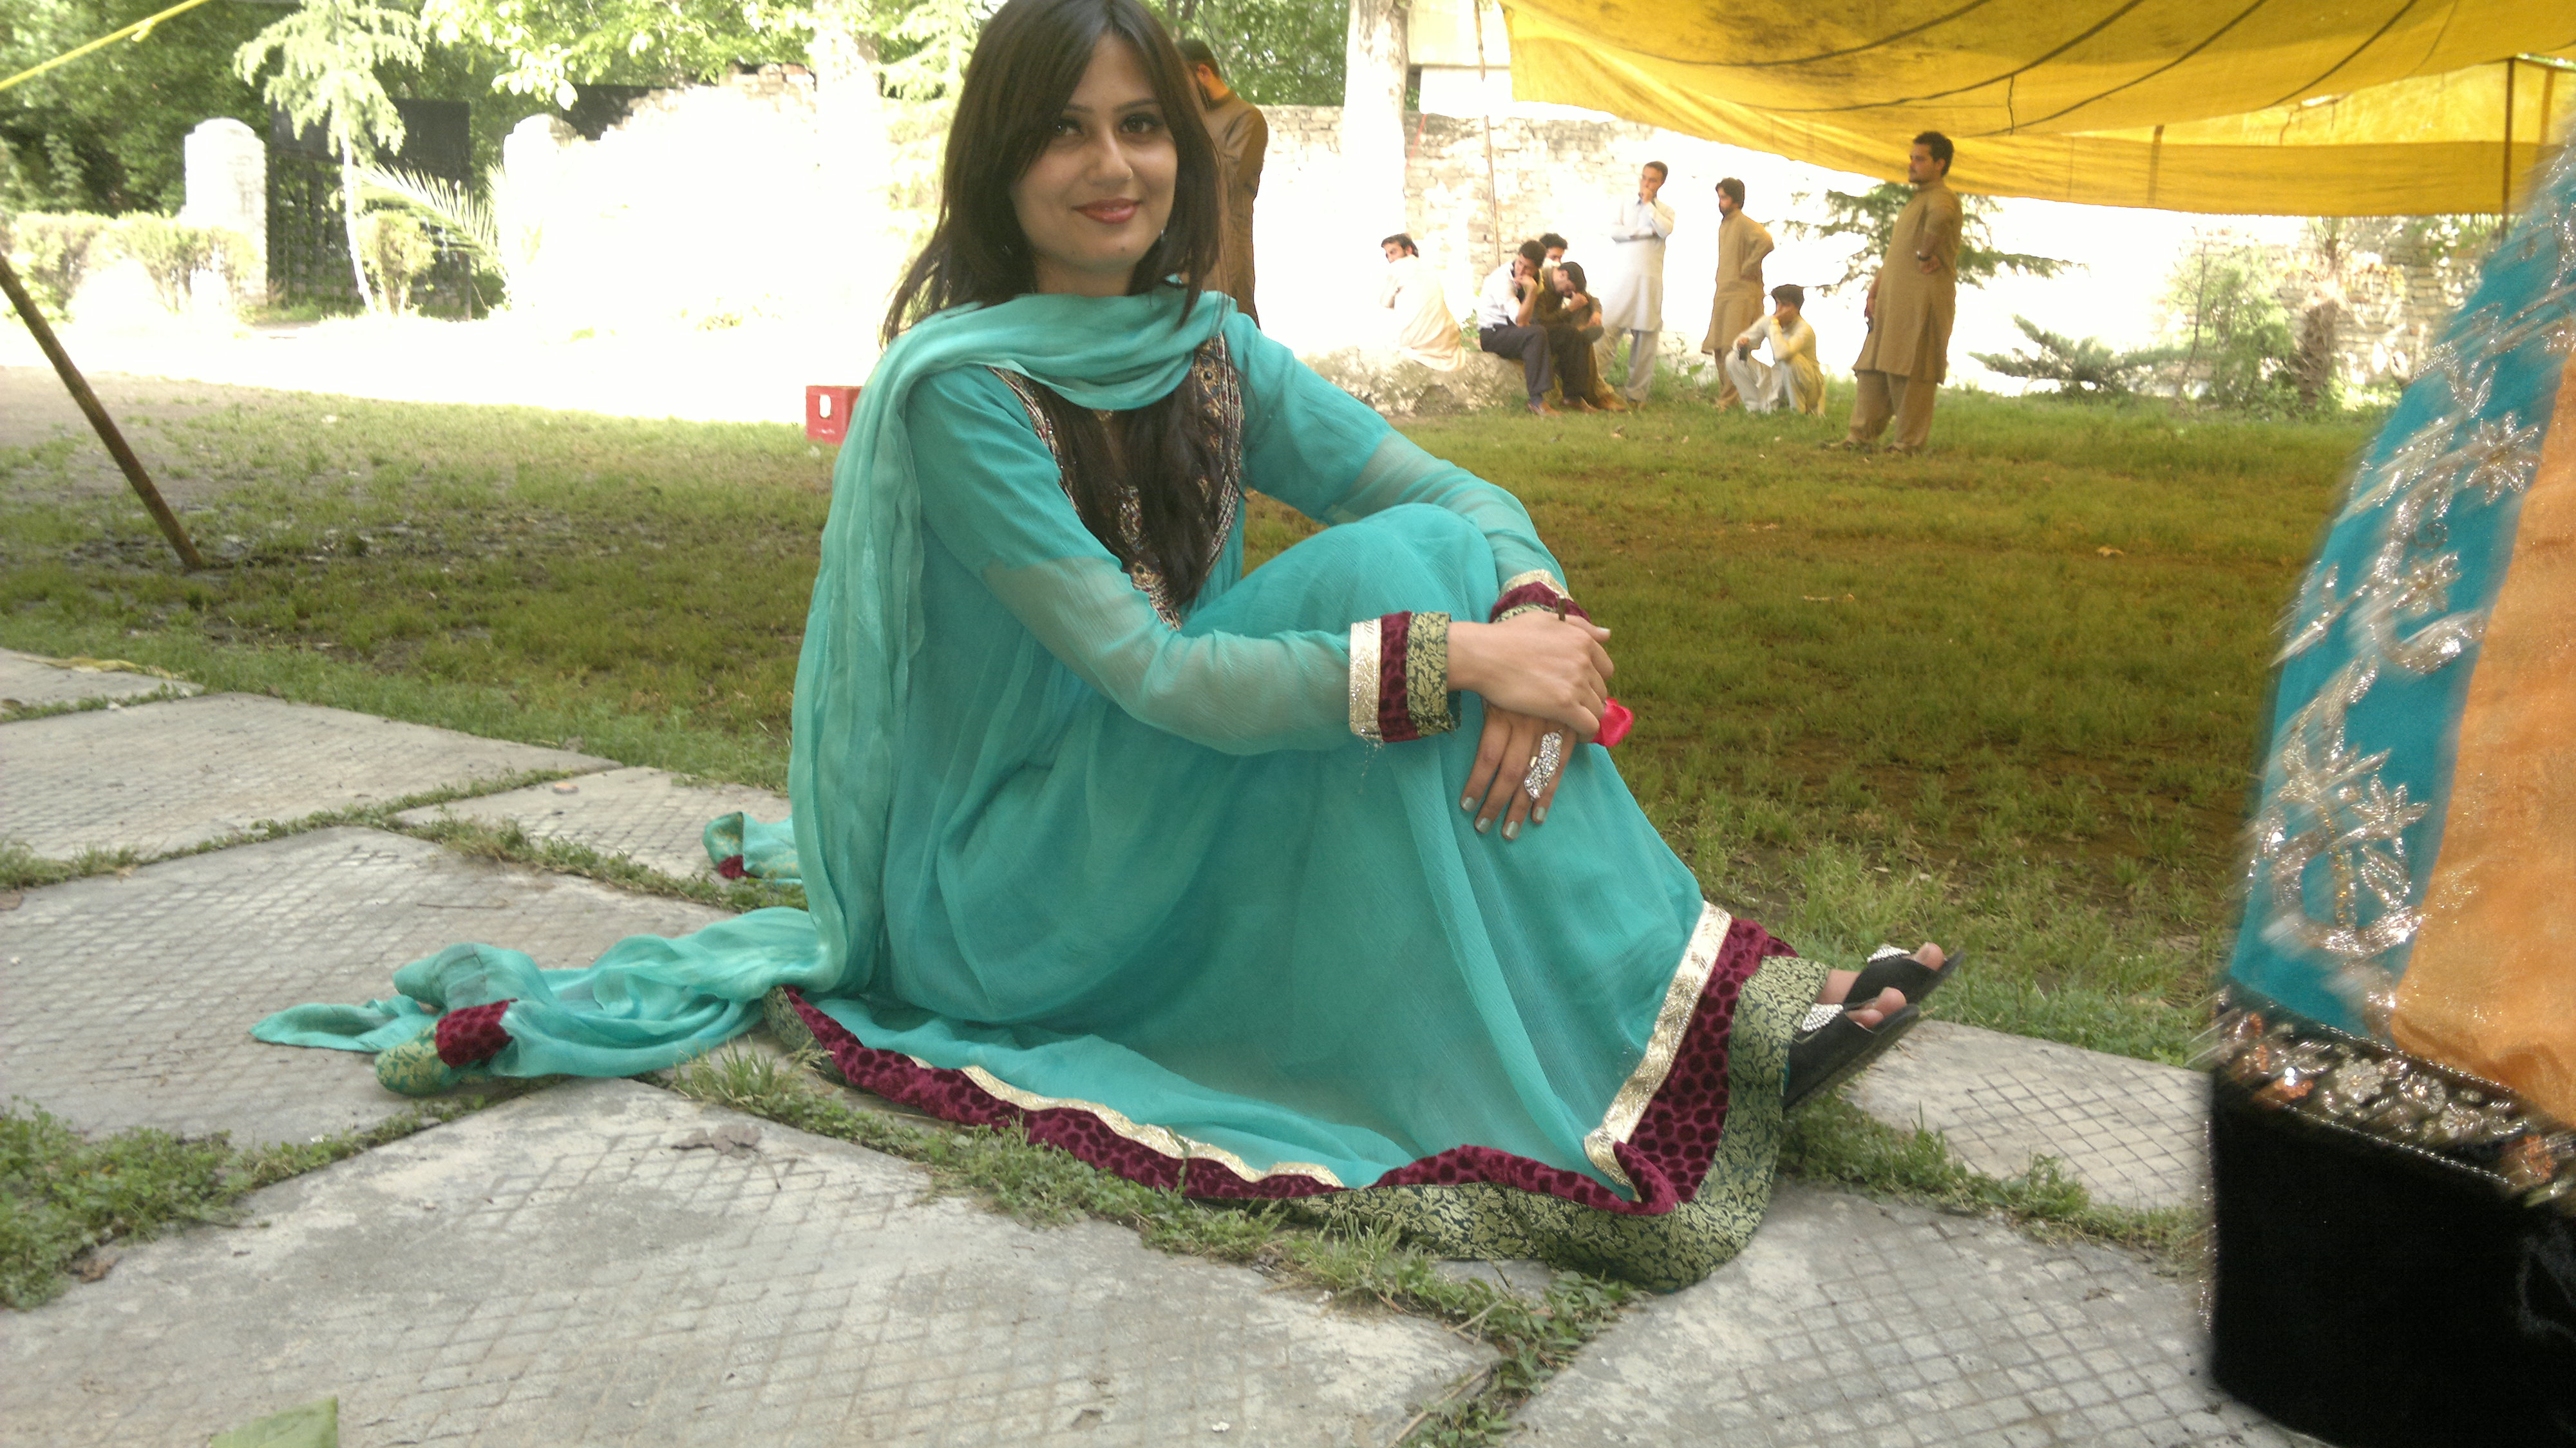
\includegraphics[width=0.6\textwidth]{/Users/asamad/Documents/programming_Coding/latex/1_first_course/myimages/zz3z.jpg}}
	\caption{A scan image}
\end{figure}










	
	
	
\end{document}